\section{Optimointimenetelmät}

Konekoodiksi kääntäminen tuo ongelmaksi hitaan käännösvaiheen. Tämän takia modernit virtuaalikoneet sisältävät useamman kuin yhden kerroksen kääntäjiä eritasoisilla optimoinneilla. Tässä luvussa esitellään muutamia keinoja, joilla JavaScript-virtuaalikoneet ovat parantaneet kääntäjien suorituskykyä sekä niiden tuottaman konekoodin tehokkuutta.

\subsection{Piiloluokat}

\textit{Piiloluokat} (hidden classes)~\cite{v8design} ovat staattisia, eli muuttumattomia luokkia, joita virtuaalikone käyttää dynaamisten JavaScript-objektien kuvaamiseen. Jos objektia muutetaan, esimerkiksi lisäämällä siihen uusi kenttä, luodaan sille uusi piiloluokka. Tämä kuulostaa järjettömältä kielen dynaamisuuden takia, mutta piiloluokkien hyödyt tulevat esiin, kun ohjelmassa on paljon samanlaisia objekteja, jotka pystyvät siten hyödyntämään samaa piiloluokkaa. Kuten kuvassa~\ref{fig:hiddenclass} näkyy.

\begin{figure}[h]
    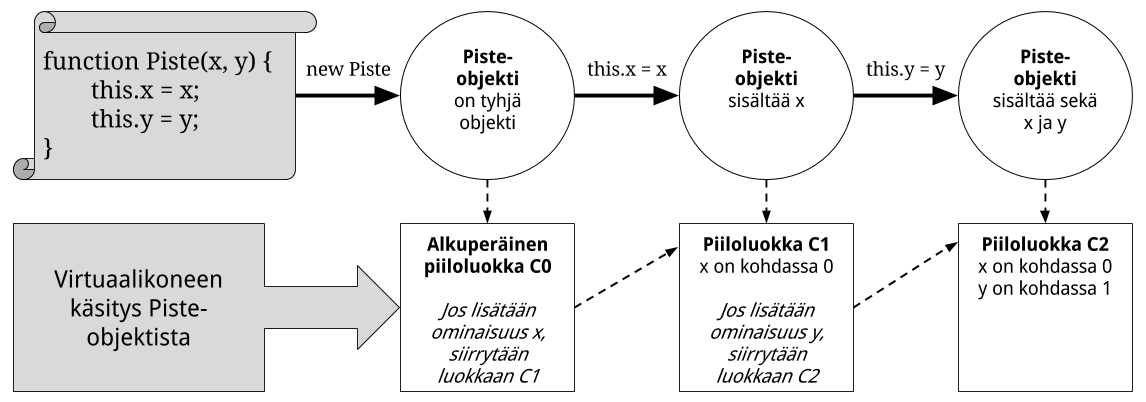
\includegraphics[width=\textwidth]{hidden-classes}
    \caption{Esimerkki piiloluokkien toimintaperiaatteesta}
     \centering
     \label{fig:hiddenclass}
\end{figure}

\subsection{Välimuistit}

(Inline cache)

\subsection{Roskienkeräys}

(Garbage collection)

\subsection{Staattinen kertasijoitusmuoto}

(Static single assignment form, SSA)